\documentclass[a4paper, ngerman]{article}
\usepackage{fancyhdr}
\usepackage[ngerman]{babel}
\usepackage{a4wide}
\usepackage{graphicx}

\renewcommand{\headrulewidth}{1pt}

\pagestyle{fancy}
\fancyhf{}

\rhead{Kapeller}
\lhead{1. Weltkrieg}

\begin{document}
\section*{Ursachen und Anlass}
\subsection*{Ursachen}
\begin{itemize}
    \item Extrem stark ausgeprägter \textbf{Nationalismus}
    \item um 1880 war Höhepunkt des \textbf{Kolonialismus}: europäische Großmächte Wettlauf nach Afrika und Asien
    \item Auf- und \textbf{Wettrüsten} von Deutschland (vorallem Flotte), der deutsche Kaiser will Engländern die Position Weltmacht Nr.1 streitig machen
    \item \textbf{Fehleinschätzung von internationalen Beziehungen} (seitens Deutschland)
          \begin{itemize}
              \item Spannungen zwischen F und GB (wegen Konkurrenz in Afrika)
              \item Deutschland rechnet nicht damit, dass sich die beiden zusammenschließen
              \item $\rightarrow$ Aufgrund von Aufrüsten von Deutschland schließen sie sich zusammen
          \end{itemize}
    \item Bereits \textbf{bestehende Konflikte}
          \begin{itemize}
              \item zwischen D und F
              \item zwischen ÖU und Russland
          \end{itemize}
    \item Sehr stark ausgeprägter \textbf{Militarismus}
          \begin{itemize}
              \item hoher Stellenwert des Militärs
              \item Politiker in Uniformen
              \item Krieg ist "normal"
              \item Militärische Ideal in Familien (Männer$>$Frauen, häusliche Gewalt, Gewalt in der Erziehung)
              \item Waffen als Spielzeug
          \end{itemize}
\end{itemize}
\subsection*{Anlass}
\begin{itemize}
    \item \textbf{28. Juni 1914}: Attentat in Sarajevo auf den österr. Thronfolger \textbf{Franz Ferdinand}
    \item Anlässlich einer österr. Militärparade
    \item Attentäter: \textbf{Gavrilo Princip} (serbischer Nationalist, Geheimorganisation Schwarze Hand)
\end{itemize}
\subsubsection*{Hintergrund}
In Vielvölkerstaat ÖU große Unzufriedenheit auf Seiten der Minderheitsvölker (in österr. Hälfte war nur Deutsch Amtssprache
, in ungarischer nur Ungarisch, ...), allgemein: \textbf{Probleme für Minderheiten im alltäglichen Leben} \\
$\rightarrow$ Minderheiten wollen sich von Habsburgmonarchie lösen und eigenen Nationalstaat bilden \\
Franz Ferdinand hatte Pläne um Probleme abzumildern: Dualismus zu Trialismus (ÖU + Serben) machen \\
\textbf{ABER} serbischer Staat will unzufriedene "österr. Serben" damit sie gegen ÖU rebellieren! \\
$\rightarrow$ Franz Ferdinand Feindbild für nationalistische Serben

\subsubsection*{Folgen}
Österreich wollte an Untersuchungen in Serbien mitarbeiten; stellte Serbien ein \textbf{Ultimatum}; drohte mit Krieg \\
Serbien ging grundsätzlich auf Forderungen ein, aber österr. Militär drängte zum Krieg (Deutschland signalisierte Unterstützung) \\
$\rightarrow$ Österreich erklärt Serbien den Krieg (\textbf{28. Juli 1914})

\section*{Bündnisblöcke}
Eigentlich dachte man es wird ein kurzer Krieg, der nur am Balkan stattfinden wird, aber militärische Bündnisverträge traten in Kraft.
\begin{center}
    \begin{tabular}{ c c }
        \textbf{Mittelmächte} & \textbf{Entente}  \\
        ÖU                    & Russland          \\
        Deutschland           & GB                \\
        Osmanisches Reich     & Frankreich        \\
        Bulgarien             & Serbien           \\
                              & Rumänien          \\
                              & Italien (ab 1915) \\
                              & USA (ab 1917)
    \end{tabular}
\end{center}
USA tritt bei u.a weil D hat uneingeschränkten U-Boot-Krieg erklärt und US-amerikanische Schiffe angegriffen hat.
\section*{Verlauf}
\begin{enumerate}
    \item \textbf{1914} | Attentat Sarajevo
    \item \textbf{1914} | Ultimatum
    \item \textbf{1914} | Mobilmachung Russlands unter Zar
    \item \textbf{1914} | Schlieffenplan (Frankreich angreifen, während Russland noch mobil macht; ging schief, weil
          Frankreich nicht rechtzeitig besiegt wurde)
    \item ...
    \item \textbf{1917} | uneingeschränkter U-Boot-Krieg
    \item \textbf{1917} | Kriegseintritt USA
    \item \textbf{1917} | Februarrevolution in Russland (Teile der Armee rebellierten; Zar verhaftet und erschossen; ABER kein Kriegsaustritt)
    \item \textbf{1917} | Oktoberrevolution in Russland (Putsch der Kommunisten; Grund für Russland aus Krieg auszutretten)
    \item \textbf{1917} | Waffenstillstand zwischen Russland und Mittelmächten
    \item \textbf{1918} | Waffenstillstand
\end{enumerate}
\section*{Kriegsende}
\subsection*{In ÖU}
\textbf{November 1918}: Kaiser Karl (Nachfolger von Franz Joseph\footnote{starb 1916}) will noch Monarchie retten aber tritt zurück und in Wien wurde die
Republik (Deutsch-Österreich) ausgerufen.
\subsection*{Friedensverträge}
\begin{itemize}
    \item Ort der Verhandlungen: Paris
    \item Die "großen Vier": USA, Frankreich, GB und Italien
    \item Vertrag von St. Germain (\textbf{Österreich})
          \begin{itemize}
              \item Gebietsverluste (k. u. k.-Monarchie zerfällt: SHS-Staat, Jugoslawien \footnote{6 Teilrepubliken:
                        Slowenien, Kroatien, Bosnien und Herzegowina, Montenegro, Serbien, Mazedonien})
              \item Burgenland von Ungarn zu Österreich
              \item Namensänderung: "Republik Deutsch-Österreich" $\rightarrow$ "Republik Österreich"
              \item Armee reduzieren
          \end{itemize}
    \item Vertrag von Versailles (\textbf{Deutschland})
          \begin{itemize}
              \item Gebietsverluste (Elsass-Lothringen wieder an Frankreich; Teile von Schlesien an Polen, ...)
              \item Abrüstung: Kriegsflotte aufgeben $\rightarrow$ Imageschaden für Militär
              \item Reparationszahlungen (Kriegsschuld \footnote{Deutschland hatte alleinige Kriegsschuld zugewiesen bekommen} begleichen)
          \end{itemize}
\end{itemize}

\begin{figure}[h]
    \centering
    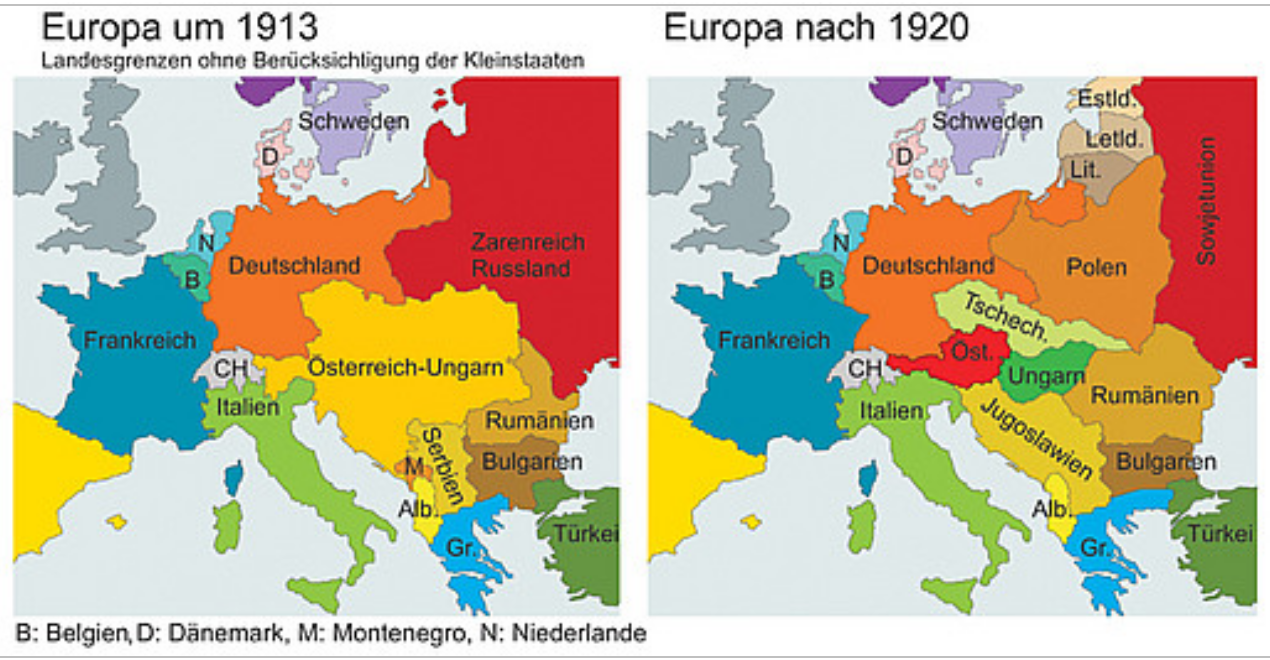
\includegraphics[scale=0.23]{eu.png}
    \caption{Europa vor und nach 1.WK}
\end{figure}

\end{document}